% =====================================================================
% Paper FDTooth — formato Springer LNCS (plantilla ESAN)
% Borrador en ESPAÑOL; la traducción al inglés se hará al final.
% Compilar: latexmk -pdf main.tex   (pdflatex + bibtex, estilo splncs04)
% Guía de redacción: GUIA_REDACCION_PAPER.md
% =====================================================================
\documentclass[runningheads]{llncs}

\usepackage[T1]{fontenc}
\usepackage[utf8]{inputenc}
\usepackage[spanish,es-tabla,es-nodecimaldot,es-nosectiondot]{babel}
\usepackage{graphicx}
\usepackage{booktabs}
\usepackage{amsmath}
\usepackage[hidelinks]{hyperref}
\usepackage{xcolor}
\graphicspath{{img/}}
\renewcommand{\keywordname}{{\bfseries Palabras clave:}}
\renewcommand{\andname}{y}
\renewcommand{\lastandname}{\unskip\ y}

% ---- Código de colores de redacción (guías del curso) -----------------
% \prob{} problema (VD) = azul   | \sol{} solución/técnica (VI) = rojo
% \dat{}  dataset/datos  = verde  | \con{} conector de adición = resaltado
% Para la versión final cambia \colorestrue por \coloresfalse.
\definecolor{problema}{RGB}{0,112,192}
\definecolor{solucion}{RGB}{192,0,0}
\definecolor{dataset}{RGB}{0,128,0}
\newif\ifcolores
\colorestrue
\ifcolores
  \newcommand{\prob}[1]{\textcolor{problema}{\textbf{#1}}}
  \newcommand{\sol}[1]{\textcolor{solucion}{\textbf{#1}}}
  \newcommand{\dat}[1]{\textcolor{dataset}{\textbf{#1}}}
  \newcommand{\con}[1]{{\setlength{\fboxsep}{0.5pt}\colorbox{yellow}{\strut #1}}}
\else
  \newcommand{\prob}[1]{#1}
  \newcommand{\sol}[1]{#1}
  \newcommand{\dat}[1]{#1}
  \newcommand{\con}[1]{#1}
\fi

\begin{document}

% Título definitivo (igual al del plan de tesis, patrón PREDICTIVO_TEMAS)
\title{Diseño de un Sistema de \sol{Visión Computacional} para el
Pre-diagnóstico de \prob{Fenestración y Dehiscencia Ósea Alveolar} a partir
de \dat{Fotografías Intraorales y Tomografías CBCT}}
\titlerunning{Pre-diagnóstico de Fenestración y Dehiscencia}

\author{José Cabrera-Ticlla\inst{1} \and Lucero Ayala-Mauricio\inst{1} \and
Wilfredo Ticona\inst{1,2}}
\authorrunning{J. Cabrera-Ticlla et al.}

\institute{Universidad ESAN, Lima, Perú\\
\email{22200150@ue.edu.pe, 22200171@ue.edu.pe, wmamani@esan.edu.pe} \and
Universidad Tecnológica del Perú, Lima, Perú\\
\email{C19404@utp.edu.pe}}

\maketitle

\begin{abstract}
% Contexto (problema) -> objetivo -> metodología (M1, M2, M3) -> resultados
% principales (Macro-F1 en la prueba retenida) -> conclusión.
La \prob{fenestración} y la \prob{dehiscencia ósea alveolar} son defectos
frecuentes en los dientes anteriores que pueden terminar en recesión
gingival y pérdida dental, y su diagnóstico depende de la \dat{CBCT}, cuyo
uso rutinario está limitado por la radiación y el tiempo que demanda. Este
trabajo propone el diseño de un sistema de \sol{visión computacional} para
el pre-diagnóstico por diente de ambos defectos a partir de
\dat{fotografías intraorales y tomografías CBCT}. Sobre el dataset
\dat{FDTooth}, con una cohorte de 217 pacientes y 2604 dientes, se
compararon tres metodologías: rasgos diseñados a mano con clasificadores
de \sol{Machine Learning}, ajuste fino de \sol{ConvNeXt V2 Tiny} y
representaciones del modelo fundacional \sol{DINOv2} con clasificadores de
\sol{Machine Learning}. La evaluación usó validación cruzada agrupada por
paciente y una prueba retenida de 43 pacientes evaluada una sola vez, con
el \textit{Macro-F1} como métrica principal.
En la validación cruzada del conjunto de desarrollo, ninguna metodología
superó 0.535 de \textit{Macro-F1} con solo la fotografía, mientras que
el ensamble de \sol{ConvNeXt V2} y rasgos diseñados de la \dat{CBCT}
alcanzó 0.810 (IC 95\,\%: 0.793--0.826) y un AUC de 0.933. La \dat{CBCT}
resultó indispensable para distinguir ambos defectos.
\textbf{[Resultado en la prueba retenida pendiente.]}
\keywords{\prob{Fenestración} \and \prob{Dehiscencia} \and \dat{CBCT} \and
\dat{Fotografía intraoral} \and \sol{Visión computacional} \and
\sol{Deep Learning} \and \sol{Machine Learning}}
\end{abstract}

\ifcolores
\noindent\fbox{\parbox{\dimexpr\linewidth-2\fboxsep-2\fboxrule}{\scriptsize
\textbf{Borrador.} \prob{Problema} \quad \sol{Solución} \quad
\dat{Dataset} \quad \con{Del mismo modo, Asimismo, Por otra parte}}}
\fi

% ---------------------------------------------------------------------
\section{Introducción}
% Embudo (guía §3): 1) problema y relevancia mundial -> 2) cifras OMS u
% otro organismo oficial -> 3) América Latina -> 4) Perú -> 5) la IA, el ML
% y el DL como respuesta, cierre con cita múltiple.
% CRITERIO DE FUENTES: artículos de 2021 en adelante y en revistas Q1.
% Única excepción: la OMS, como organismo oficial de estadísticas.

% P1. Problema y relevancia mundial
Las enfermedades bucodentales constituyen uno de los problemas de salud
pública más extendidos del mundo y, en sus etapas avanzadas, conducen a la
pérdida de piezas dentarias \cite{oms2025saludbucodental}. Entre las
alteraciones del soporte óseo de los dientes destacan la
\prob{fenestración} y la \prob{dehiscencia ósea alveolar}: la primera es un
defecto localizado del hueso alveolar que expone la raíz sin comprometer la
cresta, mientras que la segunda es la pérdida del hueso que cubre la raíz y
afecta al margen óseo \cite{liu2025fdtooth}. Estos \prob{defectos óseos
alveolares} se asocian con exposición radicular, necrosis pulpar, recesión
gingival, bolsas periodontales profundas y, en casos severos, pérdida del
diente \cite{liu2025fdtooth}; \con{además}, su presencia antes de un
tratamiento ortodóntico puede agravar el daño periodontal, por lo que deben
evaluarse antes de mover los dientes \cite{sun2022dehiscence}.

% P2. Cifras mundiales (OMS) y magnitud del problema
La Organización Mundial de la Salud (OMS) estima que cerca de 3700 millones
de personas padecen enfermedades bucodentales y que la periodontopatía grave
supera los 1000 millones de casos en el mundo; \con{asimismo}, la pérdida
total de dientes afecta a cerca del 7\,\% de las personas de 20 años o más y
al 23\,\% de las de 60 años o más \cite{oms2025saludbucodental}. En el caso
específico de la \prob{fenestración} y la \prob{dehiscencia}, su frecuencia
es elevada incluso en pacientes sin maloclusiones severas: Sun et al.
analizaron mediante \dat{tomografía computarizada de haz cónico (CBCT)} 732
dientes anteriores de 61 individuos Clase I y hallaron dehiscencia en el
27.46\,\% y fenestración en el 26.91\,\% de los dientes, con al menos un
defecto en el 48.91\,\% de ellos y en la totalidad de los pacientes
\cite{sun2022dehiscence}.

% P3. América Latina
En América Latina y el Caribe, el Estudio de la Carga Global de la
Enfermedad 2023 estimó 308.2 millones de casos prevalentes de trastornos
bucales, que ocupan el primer lugar en prevalencia entre todas las causas de
enfermedad de la región; dentro de ellos, la periodontitis severa fue el
segundo trastorno más prevalente, con 87.2 millones de casos, y su
discapacidad aumentó en 25\,\% o más desde 1990 en la mayoría de los países
\cite{gbd2026latinoamerica}. \con{Del mismo modo}, la evidencia
epidemiológica de la región se concentra en Brasil, México, Chile y
Colombia, mientras que los estudios de otros países son escasos
\cite{gbd2026latinoamerica}.

% P4. Perú
En el Perú, el mismo estudio ubica al país con la segunda tasa más alta de
años vividos con discapacidad por edentulismo en adultos de 60 años o más
de la región (1366.9 por cada 100\,000 habitantes), solo por debajo de
Bolivia \cite{gbd2026latinoamerica}. Dado que el edentulismo es el
desenlace final de la enfermedad periodontal avanzada
\cite{oms2025saludbucodental} y que la \prob{fenestración} y la
\prob{dehiscencia} pueden terminar en la pérdida del diente
\cite{liu2025fdtooth}, su detección oportuna resulta relevante para el
país; sin embargo, la evidencia peruana sobre estos defectos es
escasa \cite{gbd2026latinoamerica}.

% P5. Limitaciones del diagnóstico y la IA como respuesta
La \dat{CBCT} es la modalidad de imagen de elección para diagnosticar estos
defectos, pero su uso rutinario en los controles es poco práctico por la
exposición a radiación y el tiempo que demanda; \con{por otra parte}, la
inspección visual de las \dat{fotografías intraorales} es subjetiva, lenta
y puede ser poco precisa \cite{liu2025fdtooth}. Ante ello, la
\sol{inteligencia artificial (IA)} ha ganado participación en el
diagnóstico odontológico: un metaanálisis reciente reportó, para la
detección de periodontitis en radiografías, una sensibilidad agrupada de
0.93 y una especificidad de 0.88 a nivel de paciente
\cite{zhang2026periodontitis}, y los modelos de \sol{visión computacional}
ya permiten el cribado remoto de enfermedades bucales a partir de
\dat{imágenes intraorales} \cite{chen2026surveillance}. \con{De igual
manera}, modelos de \sol{Deep Learning} han detectado \prob{fenestración y
dehiscencia} directamente en cortes de \dat{CBCT}, con exactitudes de 0.82
a 0.95 a nivel de diente \cite{xu2026swinunetr}. \con{Asimismo}, la
publicación del dataset \dat{FDTooth}, que reúne fotografías intraorales y
CBCT de 241 pacientes, incluyó un modelo de referencia que detecta estos
defectos solo a partir de fotografías, con un AUC de 0.76 y una
especificidad de 0.65, sin distinguir entre fenestración y dehiscencia
\cite{liu2025fdtooth}. Estos resultados muestran el potencial de la IA,
pero también la necesidad de aprovechar ambas modalidades de forma
conjunta \cite{liu2025fdtooth,zhang2026periodontitis,xu2026swinunetr}.

% P6. Propósito del trabajo (sin adelantar resultados)
En este contexto, el presente trabajo propone el diseño de un sistema de
\sol{visión computacional} para el pre-diagnóstico de \prob{fenestración y
dehiscencia ósea alveolar} a partir de \dat{fotografías intraorales y
tomografías CBCT}. Para ello, se comparan tres enfoques sobre el dataset
\dat{FDTooth}: rasgos diseñados a mano con \sol{Machine Learning}, ajuste
fino de una \sol{red convolucional preentrenada} y representaciones de un
\sol{modelo fundacional} combinadas con clasificadores de \sol{Machine
Learning}.

% ---------------------------------------------------------------------
\section{Trabajos Relacionados}
% Subsecciones "[Técnica] para [problema]", una por cada metodología del
% trabajo (M1, M2, M3). Cada una es un párrafo: contexto -> Autor et al. [n]
% + técnica + datos + mejor métrica + hallazgo, enlazados con conectores, y
% una oración final de síntesis propia. Criterio: 2021+ y revistas Q1.

\subsection{\sol{Machine Learning} con rasgos diseñados a mano para el
diagnóstico de \prob{lesiones óseas dentales}}
Los clasificadores de \sol{Machine Learning} alimentados con rasgos
cuantitativos de la imagen, como los radiómicos, de textura y de color, han
sido ampliamente estudiados para el diagnóstico de \prob{lesiones de los
maxilares} en \dat{CBCT}. Song et al. \cite{song2024radiomics} extrajeron
348 rasgos radiómicos de las \dat{CBCT} de 326 pacientes para diferenciar
\prob{ameloblastoma y queratoquiste odontogénico} con seis algoritmos, y
\sol{XGBoost} alcanzó una exactitud de 0.843, un F1 de 0.841 y un AUC de
0.872, con un desempeño superior al de los radiólogos. \con{Del mismo
modo}, Sha et al. \cite{sha2025radiomics} integraron seis rasgos
radiómicos de las \dat{CBCT} de 300 pacientes en un clasificador por
votación suave que combina \sol{Random Forest, SVM y regresión logística},
y obtuvieron en el conjunto de prueba valores de AUC de 0.781 a 0.849 y una
exactitud de 0.711 al distinguir tres tipos de \prob{lesiones quísticas}.
\con{Asimismo}, centrándose en pacientes con \prob{periodontitis}, Zhang et
al. \cite{zhang2026radiomic} emplearon 206 rasgos radiómicos de
\dat{CBCT}, y el modelo \sol{Random Forest} logró un AUC de 0.710 para
detectar aterosclerosis carotídea concomitante. \con{Por otra parte},
Rashid y Dudley \cite{rashid2026cielab} transformaron mediciones de color
\dat{CIELAB} de 300 dientes extraídos en rasgos diseñados para clasificar
la severidad de la \prob{caries oclusal}, y observaron que los modelos
basados en árboles (\sol{Random Forest, XGBoost y CatBoost}) rindieron por
debajo de las redes neuronales, que alcanzaron una exactitud balanceada de
0.89, y que apenas mejoraban con más datos de entrenamiento. En conjunto,
estos trabajos muestran que los rasgos diseñados a mano son interpretables
y eficaces con muestras moderadas, pero ninguno los aplicó a la
\prob{fenestración y dehiscencia} ni a \dat{fotografías intraorales}.

\subsection{\sol{Deep Learning} para la evaluación del \prob{hueso
alveolar} en \dat{CBCT y fotografías intraorales}}
Conscientes de las limitaciones de los rasgos diseñados a mano, trabajos
recientes han aplicado \sol{Deep Learning} a la evaluación del
\prob{soporte óseo periodontal}. Tichy et al.
\cite{tichy2026periodontology} revisaron 29 estudios de \sol{Deep
Learning} para el diagnóstico de \prob{periodontitis} y reportaron
exactitudes de 81 a 99\,\% en radiografías panorámicas y de 78\,\% en
\dat{CBCT}, así como un AUROC de 0.93 en el cribado con \dat{fotografías},
aunque advirtieron que la mayoría utilizó datos de un solo centro.
\con{Del mismo modo}, Yang et al. \cite{yang2026horizontal} entrenaron una
\sol{3D-ResNet} con 505 \dat{CBCT} para clasificar la \prob{pérdida ósea
horizontal} de los primeros molares inferiores y alcanzaron una exactitud
global de 0.829, comparable a la de los odontólogos (0.820).
\con{Asimismo}, Palkovics et al. \cite{palkovics2026segmentation}
utilizaron una \sol{SegResNet} para segmentar en \dat{CBCT} los
\prob{defectos periodontales infraóseos} mandibulares, con mediciones
lineales y volumétricas confiables frente a la segmentación
semiautomática, mientras que Xu et al. \cite{xu2026swinunetr} entrenaron
un \sol{Swin UNETR} con 10\,752 cortes sagitales de \dat{CBCT} para medir
y detectar la \prob{fenestración y dehiscencia}. \con{Por otra parte}, en
el caso de las \dat{fotografías intraorales}, Mao et al.
\cite{mao2025photographs} analizaron 26 estudios de detección de
\prob{enfermedad periodontal} y hallaron exactitudes de clasificación de
0.46 a 1.00, con solo 9 estudios que usaron más de una vista. \con{De
igual manera}, Li et al. \cite{li2026transverse} compararon seis
\sol{redes convolucionales} entrenadas con \dat{fotografías intraorales
frontales} de 826 pacientes, usando como referencia mediciones derivadas
de \dat{CBCT}, y \sol{ResNet-18} alcanzó una exactitud de 90.62\,\% en un
conjunto de prueba externo para detectar la \prob{deficiencia transversal
maxilar}. Estos resultados confirman que un modelo basado en fotografías
puede aprender de etiquetas obtenidas por \dat{CBCT}, aunque el desempeño
varía según la tarea y la vista utilizada.

\subsection{\sol{Modelos fundacionales y fusión multimodal} en el
\prob{diagnóstico odontológico}}
Ante la escasez de datos etiquetados, los \sol{modelos fundacionales}
preentrenados de forma autosupervisada y la \sol{fusión multimodal} se
perfilan como alternativas al entrenamiento supervisado desde cero. Hu et
al. \cite{hu2025selfsupervised} adaptaron \sol{DINOv2} mediante
aprendizaje autosupervisado específico del dominio para segmentar
\dat{radiografías periapicales} con pocas anotaciones, y lograron un Dice
de 74.77\,\% frente a 33.53--41.55\,\% de U-Net y DeepLabV3+, superando
también a MAE, MoCo v3 y BEiT v3. \con{Del mismo modo}, Li et al.
\cite{li2025hcnet} preentrenaron y ajustaron el modelo \sol{HC-Net+} con
10\,881 \dat{ortopantomografías} para detectar \prob{periodontitis} en
estadios II a IV, superaron a los periodoncistas (AUROC de 94.2\,\% frente
a 85.6\,\%) y mantuvieron una exactitud superior a 92.4\,\% en cuatro
centros. \con{Asimismo}, Feng et al. \cite{feng2026multimodal} revisaron
la \sol{fusión de datos multimodales} en ortodoncia y concluyeron que
integrar modalidades compensa las limitaciones de resolución y de
especificidad tisular que presenta cada una por separado. \con{Por otra
parte}, Chen et al. \cite{chen2026surveillance} señalaron que los modelos
multimodales permiten integrar imágenes y datos clínicos en la vigilancia
de la salud bucal. Sin embargo, el único trabajo que aborda la
\prob{fenestración y dehiscencia} con \dat{fotografías intraorales}
pareadas con \dat{CBCT}, el de Liu et al. \cite{liu2025fdtooth}, empleó un
ensamble de \sol{redes convolucionales} supervisadas solo sobre la
fotografía y en una tarea binaria. Hasta donde se conoce, no se ha
evaluado un \sol{modelo fundacional} ni la \sol{fusión} de ambas
modalidades para distinguir por diente entre normal, \prob{fenestración} y
\prob{dehiscencia}, vacío que aborda el presente trabajo.

% ---------------------------------------------------------------------
\section{Metodología}
% Una subsección por bloque de la figura (img/metodologia.png). Tres
% metodologías comparadas: M1 (gris) rasgos diseñados a mano + ML;
% M2 (azul) ajuste fino de ConvNeXt V2 Tiny; M3 (verde) DINOv2 ViT-B/14 + ML.
La Fig.~\ref{fig:metodologia} resume la metodología propuesta.

\begin{figure}[t]
\centering
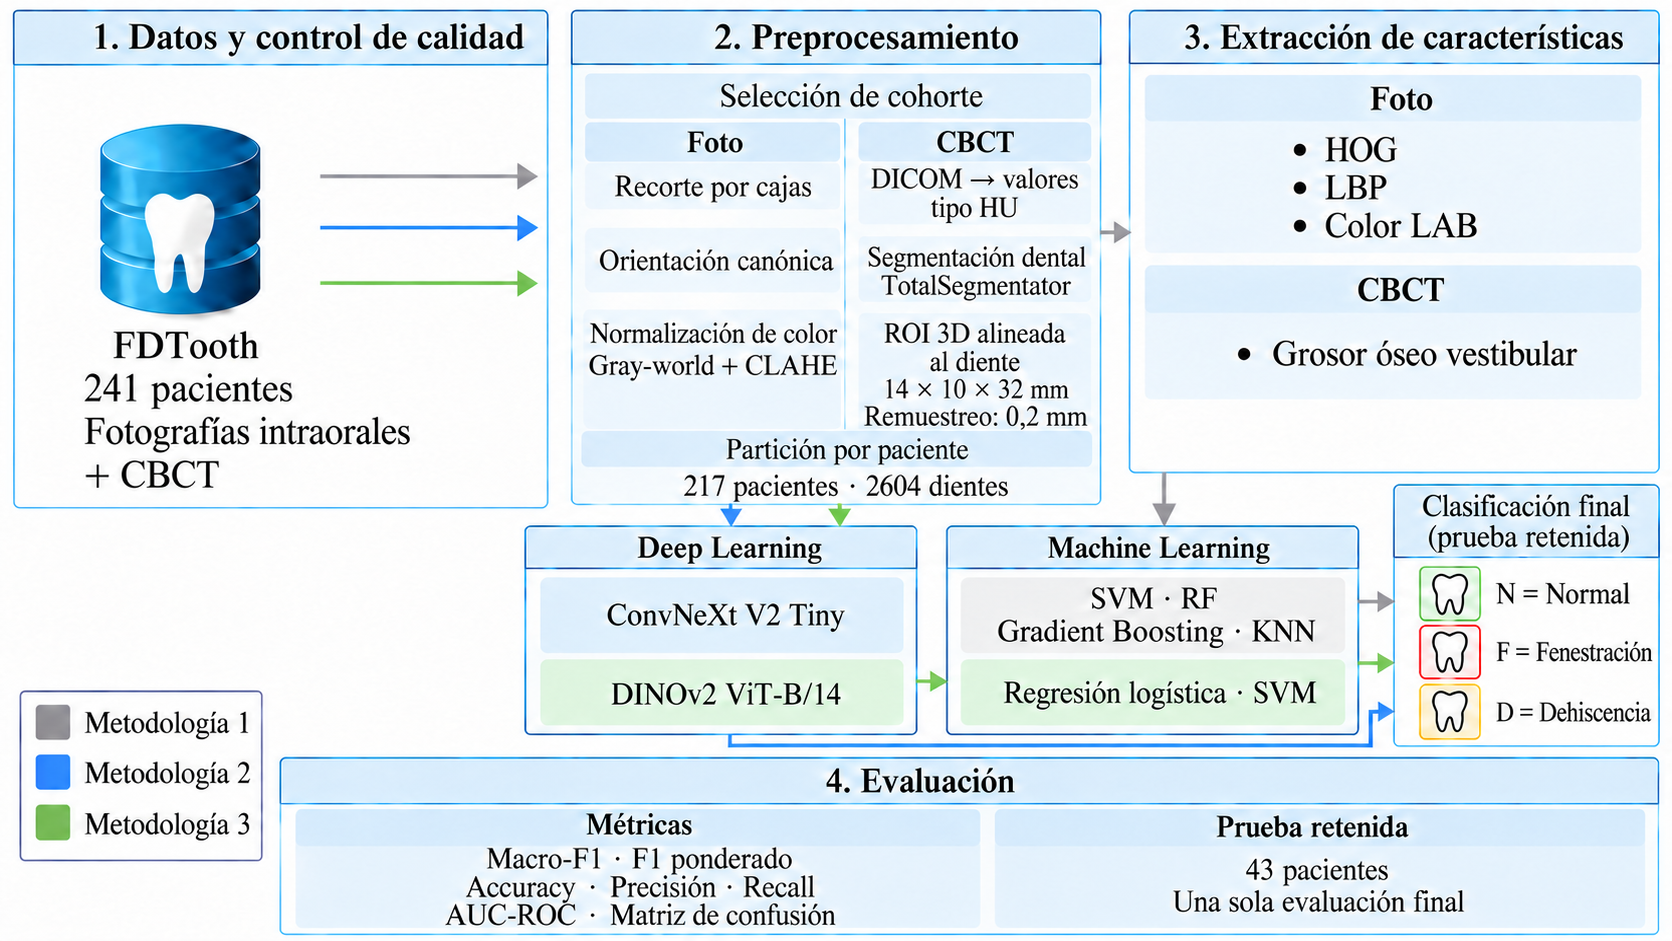
\includegraphics[width=\textwidth]{metodologia.png}
\caption{Metodología.}
\label{fig:metodologia}
\end{figure}

\subsection{Datos y control de calidad}
% Bloque 1 de la figura.
Se utilizó el dataset público \dat{FDTooth} \cite{liu2025fdtooth},
recolectado entre enero de 2010 y enero de 2023 en dos centros de la
Facultad de Odontología de la Universidad de Hong Kong. Para cada uno de
sus 241 pacientes, de 9 a 55 años, el dataset incluye una \dat{fotografía
intraoral frontal} en formato JPEG de $5760 \times 3840$ píxeles y una
\dat{tomografía CBCT} en formato DICOM con un tamaño de vóxel de 0.15 a
0.18 mm. Cada uno de los 12 dientes anteriores tiene una etiqueta de
referencia: normal (N), \prob{fenestración} (F) o \prob{dehiscencia} (D).
Esta etiqueta proviene de la lectura de la \dat{CBCT} por dos odontólogos
experimentados, con una concordancia $\kappa > 0.9$
\cite{liu2025fdtooth}. Antes del modelado, se verificó la integridad de
los 487 archivos mediante sumas SHA256 y se contrastaron las etiquetas del
archivo CSV con las del archivo JSON de anotaciones dentales. Se
excluyeron 24 pacientes: 23 por discordancia entre ambas fuentes y uno por
coordenadas de cajas incompatibles con la imagen. La cohorte apta quedó
conformada por 217 pacientes y 2604 dientes.

\subsection{Preprocesamiento}
% Bloque 2 de la figura.
En la \dat{fotografía intraoral}, cada diente se recortó a partir de su
caja delimitadora, ampliada hacia la encía para incluir el margen
gingival. El recorte se llevó a una orientación canónica y se redimensionó
a 768 píxeles en su lado largo sin deformar la imagen. Luego se normalizó
el color con el método \sol{Gray-world}, que corrige el balance de
blancos, y con \sol{CLAHE}, que realza el contraste local.
\con{Asimismo}, la \dat{CBCT} se convirtió de DICOM a valores tipo
unidades Hounsfield y se segmentó con \sol{TotalSegmentator}
\cite{wasserthal2023totalsegmentator}, que identifica cada diente según la
numeración FDI y logró segmentar 2600 de los 2604 dientes. A partir de
cada segmentación se extrajo una región de interés (ROI) 3D de
$14 \times 10 \times 32$ mm, alineada con el eje longitudinal del diente y remuestreada a vóxeles
isotrópicos de 0.2 mm. Por último, la cohorte se particionó por paciente,
de modo que todos los dientes de una persona pertenecen al mismo
conjunto: el conjunto de desarrollo reúne 174 pacientes (2088 dientes) y
el de prueba retenida, 43 pacientes (516 dientes).

\subsection{Extracción de características}
% Bloque 3 de la figura (M1).
La metodología M1 representa cada diente con un vector de rasgos
diseñados a mano. En la \dat{fotografía}, el histograma de gradientes
orientados (\sol{HOG}), reducido con análisis de componentes principales,
describe la forma del contorno gingival y la prominencia radicular.
\con{Del mismo modo}, los patrones binarios locales uniformes (\sol{LBP})
describen la textura de la superficie, y las estadísticas de color en el
espacio \sol{LAB} se calculan por separado para el diente y la encía. En
la \dat{CBCT}, se mide el perfil de \prob{grosor óseo vestibular} a lo
largo de la raíz. De este perfil se derivan la altura de la cresta ósea,
las zonas sin hueso y el grosor medio, rasgos que reflejan directamente la
diferencia entre una \prob{dehiscencia}, que compromete el margen óseo, y
una \prob{fenestración}, que deja intacta la cresta. El vector final
concatena estos rasgos con la posición del diente en la arcada.

\subsection{Modelado y clasificación}
% M1 (gris), M2 (azul), M3 (verde).
Se compararon tres metodologías, todas con la misma salida por diente: N,
F o D. En la M1, el vector de rasgos alimenta cuatro clasificadores de
\sol{Machine Learning}: \sol{SVM} con kernel RBF, \sol{Random Forest},
\sol{Gradient Boosting} y \sol{KNN}. La imputación y el escalado de los
rasgos se ajustan solo con los datos de entrenamiento de cada partición.
En la M2, se realiza el ajuste fino de la red convolucional preentrenada
\sol{ConvNeXt V2 Tiny} \cite{woo2023convnextv2} con tres entradas
alternativas: la \dat{fotografía}, una representación 2.5D de la ROI de la
\dat{CBCT} y la fusión de ambas en una arquitectura de dos ramas. El
entrenamiento emplea aumento de datos y parada temprana. \con{Por otra
parte}, en la M3 el modelo fundacional \sol{DINOv2 ViT-B/14}
\cite{oquab2023dinov2}, ya aplicado con éxito a imágenes dentales
\cite{hu2025selfsupervised}, se usa como extractor congelado. Sus
embeddings de la \dat{fotografía} y de la \dat{CBCT} se reducen con
análisis de componentes principales y se clasifican con
\sol{regresión logística} y \sol{SVM} con kernel RBF.
Por último, se evaluó un ensamble que combina las predicciones de M2 con
\dat{fusión}, M2 con \dat{CBCT} y M1 con \dat{CBCT}.

\subsection{Evaluación}
% Bloque 4 de la figura.
En el conjunto de desarrollo se aplicó una validación cruzada de cinco
particiones externas agrupadas por paciente. Dentro de cada partición de
entrenamiento, una validación interna selecciona los hiperparámetros, y
las predicciones fuera de partición (OOF) permiten comparar las
configuraciones sin usar el conjunto de prueba. El desempeño se mide con
\textit{Macro-F1}, F1 ponderado, exactitud (\textit{accuracy}),
precisión, sensibilidad (\textit{recall}), AUC-ROC uno contra el resto y
la matriz de confusión. La métrica principal es el \textit{Macro-F1},
porque pondera por igual las tres clases y no premia a un modelo que solo
acierta la clase mayoritaria.
Los intervalos de confianza del 95\,\% y las diferencias entre modelos
se estimaron mediante \textit{bootstrap} de pacientes con 1000 a 2000
remuestreos. Finalmente, la mejor configuración de cada
metodología se reentrena con todo el conjunto de desarrollo y se evalúa
una sola vez en la prueba retenida de 43 pacientes (516 dientes).

% ---------------------------------------------------------------------
\section{Resultados}
% Tablas: leyenda ENCIMA. Figuras: leyenda DEBAJO.
% ESTADO: resultados preliminares del conjunto de desarrollo (OOF). Falta la
% prueba retenida (43 pacientes, 516 dientes) tras el entrenamiento final de M2.
Los resultados corresponden a las predicciones fuera de partición del
conjunto de desarrollo, que reúne 174 pacientes y 2088 dientes: 938
normales, 663 con \prob{fenestración} y 487 con \prob{dehiscencia}. Los
intervalos de confianza (IC) del 95\,\% se estimaron por remuestreo
\textit{bootstrap} de pacientes. \textbf{[Resultados en la prueba retenida
pendientes.]}

\subsection{Comparación por metodología y modalidad}
La Tabla~\ref{tab:modalidad} resume el mejor modelo de cada metodología
según la modalidad de entrada. Con solo la \dat{fotografía intraoral},
ninguna metodología superó un \textit{Macro-F1} de 0.535, valor cercano al
del enfoque de referencia basado solo en fotografías (0.55). En cambio, al
incorporar la \dat{CBCT} el desempeño subió a un rango de 0.621 a 0.789, y
\sol{ConvNeXt V2 Tiny} con ajuste fino (M2) obtuvo los mejores valores en
la \dat{CBCT} (0.789) y en la \dat{fusión} (0.796). El ensamble de M2 con
\dat{fusión}, M2 con \dat{CBCT} y M1 con \dat{CBCT} alcanzó el mejor
resultado global, con un \textit{Macro-F1} de 0.810.

\begin{table}[t]
\centering
\caption{\textit{Macro-F1} del mejor modelo de cada metodología por
modalidad (conjunto de desarrollo).}
\label{tab:modalidad}
\begin{tabular}{lcccc}
\toprule
Modalidad & Referencia$^{a}$ & M1 rasgos & M3 DINOv2 & M2 ConvNeXt V2 \\
\midrule
Fotografía & 0.55 & 0.535 & 0.510 & 0.534 \\
CBCT & -- & 0.741 & 0.621 & 0.789 \\
Fusión & -- & 0.715 & 0.598 & 0.796 \\
\midrule
\multicolumn{4}{l}{Ensamble (M2 fusión + M2 CBCT + M1 CBCT)} & \textbf{0.810} \\
\bottomrule
\multicolumn{5}{l}{\scriptsize $^{a}$ Enfoque del antecedente \cite{liu2025fdtooth}, basado solo en fotografías, en la tarea de tres clases.}
\end{tabular}
\end{table}

\subsection{Desempeño de los modelos principales}
La Tabla~\ref{tab:metricas} detalla las métricas de los modelos
principales. El ensamble obtuvo un \textit{Macro-F1} de 0.810 (IC 95\,\%:
0.793--0.826), una exactitud de 0.816 y un AUC de 0.933, con valores de F1
equilibrados entre las tres clases: 0.852 para normal, 0.784 para
\prob{fenestración} y 0.793 para \prob{dehiscencia}. \con{Asimismo}, su
sensibilidad fue de 0.832, 0.805 y 0.801, y su precisión de 0.873, 0.764 y
0.786 para las clases N, F y D, respectivamente. Entre los modelos
individuales, M2 con \dat{fusión} (0.796) y M2 con \dat{CBCT} (0.789)
superaron a \sol{Random Forest} con rasgos de la \dat{CBCT} (0.741),
mientras que \sol{DINOv2} con \sol{regresión logística} no pasó de 0.621.

\begin{table}[t]
\centering
\caption{Métricas de los modelos principales (conjunto de desarrollo). El
AUC es el promedio macro uno contra el resto.}
\label{tab:metricas}
\setlength{\tabcolsep}{3pt}
\resizebox{\textwidth}{!}{%
\begin{tabular}{llcccccccc}
\toprule
Modelo & Modalidad & Macro-F1 [IC 95\,\%] & F1 pond. & Exact. & AUC & F1 N & F1 F & F1 D \\
\midrule
\textbf{Ensamble} & Fusión & \textbf{0.810} [0.793, 0.826] & 0.817 & 0.816 & 0.933 & 0.852 & 0.784 & 0.793 \\
M2 ConvNeXt V2 & Fusión & 0.796 [0.778, 0.814] & 0.803 & 0.801 & 0.921 & 0.838 & 0.765 & 0.786 \\
M2 ConvNeXt V2 & CBCT & 0.789 [0.770, 0.805] & 0.795 & 0.795 & 0.909 & 0.832 & 0.758 & 0.776 \\
M2 ConvNeXt V2 & Foto & 0.534 [0.506, 0.561] & 0.542 & 0.540 & 0.724 & 0.590 & 0.490 & 0.523 \\
M1 Random Forest & CBCT & 0.741 [0.715, 0.763] & 0.751 & 0.750 & 0.889 & 0.807 & 0.699 & 0.715 \\
M1 Random Forest & Fusión & 0.715 [0.691, 0.740] & 0.729 & 0.728 & 0.878 & 0.789 & 0.684 & 0.673 \\
M1 Random Forest & Foto & 0.535 [0.505, 0.562] & 0.544 & 0.541 & 0.723 & 0.599 & 0.479 & 0.526 \\
M3 DINOv2 + RL & CBCT & 0.621 [0.596, 0.645] & 0.632 & 0.630 & 0.804 & 0.685 & 0.583 & 0.596 \\
M3 DINOv2 + SVM & Fusión & 0.598 [0.571, 0.625] & 0.612 & 0.613 & 0.797 & 0.675 & 0.563 & 0.557 \\
M3 DINOv2 + SVM & Foto & 0.510 [0.480, 0.540] & 0.528 & 0.532 & 0.718 & 0.622 & 0.432 & 0.477 \\
\bottomrule
\multicolumn{9}{l}{RL: regresión logística. Exact.: exactitud. F1 pond.: F1 ponderado.}
\end{tabular}}
\end{table}

\subsection{Análisis de errores}
La Tabla~\ref{tab:confusion} compara las matrices de confusión del
ensamble y de M1 con \dat{CBCT}. En el ensamble, el error más frecuente fue
clasificar dientes normales como \prob{fenestración} (111 casos), mientras
que la confusión entre \prob{fenestración} y \prob{dehiscencia} se redujo
de 107 a 59 dientes en el sentido F$\rightarrow$D y de 60 a 54 en el
sentido D$\rightarrow$F con respecto a M1. \con{Del mismo modo}, al agrupar
ambos defectos en una sola clase patológica, M2 con \dat{fusión} alcanzó
una sensibilidad de 0.927, una especificidad de 0.774, una exactitud de
0.858 y un AUC de 0.925, y entre los dientes patológicos distinguió la
\prob{fenestración} de la \prob{dehiscencia} con una exactitud de 0.873.

\begin{table}[t]
\centering
\caption{Matrices de confusión en el conjunto de desarrollo (filas: clase
real; columnas: clase predicha).}
\label{tab:confusion}
\begin{tabular}{lccc@{\hspace{8mm}}ccc}
\toprule
& \multicolumn{3}{c}{Ensamble} & \multicolumn{3}{c}{M1 RF (CBCT)} \\
\cmidrule(lr){2-4}\cmidrule(lr){5-7}
Real & N & F & D & N & F & D \\
\midrule
N (938) & 780 & 111 & 47 & 740 & 142 & 56 \\
F (663) & 70 & 534 & 59 & 91 & 465 & 107 \\
D (487) & 43 & 54 & 390 & 65 & 60 & 362 \\
\bottomrule
\end{tabular}
\end{table}

\subsection{Comparaciones estadísticas}
La diferencia de \textit{Macro-F1} entre M2 con \dat{fusión} y M1 con
\dat{CBCT} fue de +0.056 (IC 95\,\%: +0.031 a +0.080), por lo que el ajuste
fino superó de forma significativa a los rasgos diseñados a mano. En
cambio, la ventaja de la \dat{fusión} sobre la \dat{CBCT} sola dentro de M2
fue de +0.008, con un intervalo que incluye el cero, y por tanto no fue
significativa. Por último, el ensamble superó a M2 con \dat{fusión} por
+0.014 (IC 95\,\%: +0.002 a +0.025), una mejora pequeña pero
significativa.

\subsection{Discusión}
El principal hallazgo es que la \dat{CBCT} determina el desempeño: con
solo la \dat{fotografía} ninguna metodología superó 0.535 de
\textit{Macro-F1}, lo que concuerda con el desempeño moderado que reportó
el antecedente al usar solo fotografías \cite{liu2025fdtooth}. Esto
sugiere que la fotografía muestra signos indirectos de los defectos, como
el contorno gingival, pero no basta para distinguir con fiabilidad entre
\prob{fenestración} y \prob{dehiscencia}. \con{Asimismo}, el ajuste fino de
\sol{ConvNeXt V2} superó a los rasgos diseñados a mano, en línea con la
ventaja de las redes neuronales sobre los modelos basados en árboles
observada en otros problemas dentales \cite{rashid2026cielab}. \con{Por
otra parte}, \sol{DINOv2} congelado tuvo el peor desempeño con la
\dat{CBCT}. A diferencia del trabajo de Hu et al.
\cite{hu2025selfsupervised}, que adaptó \sol{DINOv2} al dominio dental
antes de usarlo, en este estudio sus representaciones, aprendidas con
imágenes naturales, se usaron sin ajuste, lo que explicaría su menor
rendimiento en cortes tomográficos. \con{De igual manera}, la
\dat{fusión} aportó una mejora marginal y no significativa sobre la
\dat{CBCT} sola, por lo que la complementariedad entre modalidades que
describe la literatura \cite{feng2026multimodal} no se tradujo aquí en una
ganancia clara. La principal limitación es que estos resultados provienen
de la validación cruzada del conjunto de desarrollo de un único dataset,
recolectado en una sola institución, por lo que falta confirmarlos en la
prueba retenida y en datos externos.

% ---------------------------------------------------------------------
\section{Conclusiones}
% BORRADOR basado en resultados de desarrollo. Actualizar con la prueba
% retenida antes de entregar.
Este trabajo diseñó un sistema de \sol{visión computacional} para el
pre-diagnóstico por diente de \prob{fenestración y dehiscencia ósea
alveolar} a partir de \dat{fotografías intraorales y tomografías CBCT}, y
comparó tres metodologías sobre el dataset \dat{FDTooth}. En la validación
cruzada del conjunto de desarrollo, el ensamble basado en el ajuste fino
de \sol{ConvNeXt V2} y en rasgos diseñados a mano de la \dat{CBCT} alcanzó
un \textit{Macro-F1} de 0.810 y un AUC de 0.933, con un desempeño
equilibrado en las tres clases. Los resultados muestran que la \dat{CBCT}
es indispensable para separar ambos defectos, que el ajuste fino supera de
forma significativa a los rasgos diseñados a mano y que un modelo
fundacional congelado no se adapta bien a las imágenes tomográficas.
\textbf{[Conclusión sobre la prueba retenida pendiente.]}

Como trabajo futuro, se propone evaluar el sistema en datos de otras
instituciones, adaptar \sol{DINOv2} al dominio de la \dat{CBCT} mediante
aprendizaje autosupervisado y explorar estrategias de fusión que aprovechen
mejor la información de la \dat{fotografía intraoral}.

% ---------------------------------------------------------------------
\bibliographystyle{splncs04unsrt} % splncs04 numerado por orden de aparición
\bibliography{referencias}

\end{document}
